\documentclass[]{article}
\usepackage[margin = 1.5in]{geometry}
\setlength{\parindent}{0in}
\usepackage{amsfonts}
\usepackage{amssymb}
\usepackage{hyperref}
\usepackage{amsmath}
\usepackage{amsthm}
\usepackage{tikz}
\usepackage[lined]{algorithm2e}
\usepackage[T1]{fontenc}
\usepackage{ae,aecompl}

\theoremstyle{definition}
\newtheorem{defn}{Definition}[section]
\newtheorem{ex}{Example}[section]

\setlength{\marginparwidth}{1.5in}
\newcommand{\lecture}[1]{\marginpar{{\footnotesize $\leftarrow$ \underline{#1}}}}

\begin{document}
	
	\title{\bf{CS 241: Foundations of Sequential Programs}}
	\date{Winter 2013, University of Waterloo \\ \center Notes written from Gordon Cormack's lectures.}
	\author{Chris Thomson}
	\maketitle
	\newpage

	\section{Introduction \& Character Encodings} 
		\lecture{January 7, 2013}
	
		\subsection{Course Structure}
		The grading scheme is 50\% final, 25\% midterm, and 25\% assignments. There are eleven assignments. Don't worry about any textbook. See the \href{https://www.student.cs.uwaterloo.ca/~cs241/W2013.pdf}{course syllabus} for more information.
		
		\subsection{Abstraction}
	
		\textbf{Abstraction} is the process of removing or hiding irrelevant details. Everything is just a sequence of bits (binary digits). There are two possible values for a bit, and those values can have arbitrary labels such as:
		\begin{itemize}
			\item Up / down.
			\item Yes / no.
			\item 1 / 0.
			\item On / off.
			\item Pass / fail.
		\end{itemize}
		
		Let's say we have four projector screens, each representing a bit of up/down, depending on if the screen has been pulled down or left up (ignoring states between up and down). These screens are up or down independently. There are sixteen possible combinations:
		\begin{center}
			\begin{tabular}{cccc}
				\underline{Screen 1} & \underline{Screen 2} &\underline{Screen 3} & \underline{Screen 4} \\
				Up (1) & Down (0) & Up (1) & Down (0) \\
				Down (0) & Down (0) & Down (0) & Up (1) \\
				\vdots & \vdots & \vdots & \vdots \\
			\end{tabular}	
		\end{center}
	
		Note that there are sixteen combinations because $k = 4$, and there are always $2^k$ combinations since there are two possible values for each of $k$ screens.
	
		\subsection{Endianness}
			Let's consider the sequence $1010$. This sequence of bits has a different interpretation when following different conventions.
			\begin{itemize}
				\item \textbf{Unsigned, little-endian}: $(1 \times 2^0) + (0 \times 2^1) + (1 \times 2^2) + (0 \times 2^3) = 1 + 4 = 5$.
				\item \textbf{Unsigned, big-endian}: $(0 \times 2^0) + (1 \times 2^1) + (0 \times 2^2) + (1 \times 2^3) = 2 + 8 = 10$.
				\item \textbf{Two's complement, little-endian}: $5 - 16 = -10$.
				\item \textbf{Two's complement, big-endian}: $10 - 16 = -6$.
				\item \textbf{Computer terminal}: LF (line feed).
			\end{itemize}
	
			Note that a two's complement number $n$ will satisfy $-2^{k-1} \le n < 2^{k-1}$.
	
		\subsection{ASCII}
	
			\textbf{ASCII} is a set of meanings for 7-bit sequences.
		
			\begin{center}
				\begin{tabular}{cc}
					\underline{Bits} & \underline{ASCII Interpretation} \\
					$0001010$ & LF (line feed) \\
					$1000111$ & G \\
					$1100111$ & g \\
					$0111000$ & 8
				\end{tabular}
			\end{center}
			
			In the latter case, $0111000$ represents the character `$8$', not the unsigned big- or little-endian number $8$. \\ \\
			ASCII was invented to communicate text. ASCII can represent characters such as A-Z, a-z, 0-9, and control characters like ();!. Since ASCII uses 7 bits, $2^7 = 128$ characters can be represented with ASCII. As a consequence of that, ASCII is basically only for Roman, unaccented characters, although many people have created their own variations of ASCII with different characters.
	
		\subsection{Unicode}
			\textbf{Unicode} was created to represent more characters. Unicode is represented as a 32-bit binary number, although representing it using 20 bits would also be sufficient. The ASCII characters are the first 128, followed by additional symbols.
			\\ \\
			A 16-bit representation of Unicode is called \textbf{UTF-16}. However, there's a problem: we have \emph{many} symbols ($> 1M$) but only $2^16 = 65,536$ possibilities to represent them. Common characters are represented directly, and there is also a `see attachment' bit for handling the many other symbols that didn't make the cut to be part of the $65,536$. Similarly, there is an 8-bit representation of Unicode called \textbf{UTF-8}, with the ASCII characters followed by additional characters and a `see attachment' bit.
			\\ \\
			The bits themselves do not have meaning. Their meaning is in your head -- everything is up for interpretation.
		\subsection{A Message for Aliens} \lecture{January 9, 2013}
			In a computer, meaning is in the eye of the beholder. We must agree on a common interpretation -- a convention. However, the English language and numbers also have their meaning determined by a set of conventions.
			\\ \\
			NASA wanted to be able to leave a message for aliens on a plaque on their spacecraft, however it was clear that aliens would not understand our language or even 0s and 1s. NASA wanted their message to be a list of prime numbers. They decided they would use binary to represent the numbers, but since 0s and 1s would be ambiguous to aliens, they used a dash (-) instead of 0, and 1 for 1. It's only a convention, but it's one that NASA determined aliens would have a higher chance of understanding.
		\subsection{Hexadecimal}
			Hexadecimal (hex) is base 16. It has sixteen case-insensitive digits: 0, 1, 2, 3, 4, 5, 6, 7, 8, 9, a, b, c, d, e, and f.
			\\ \\
			Why is hex useful? It makes conversions easy. We group bits into sequences of four:
			\begin{align*}
			  \underbrace{\underbrace{0011}_{3} \underbrace{1010}_{\text A}}_{\text{3A}}
			\end{align*}

			Conversions are made especially easy when the sequences of bits are lengthy:
			\begin{align*}
			  \underbrace{\underbrace{10}_{2} \underbrace{1110}_{\text E} \underbrace{0111}_{7} \underbrace{0011}_{3} \underbrace{1011}_{\text B} \underbrace{1001}_{9} \underbrace{1000}_{8} \underbrace{0011}_{3}}_{\text{2E73B983}}
			\end{align*}
	\section{Stored Program Computers}
		Stored program computers are also known as the \textbf{Von Neumann architecture}. They group bits into standard-sized sequences. 
		\\ \\
		In modern times, standard-sized sequences of bits are:
		\begin{itemize}
			\item \textbf{Bytes}. A byte is 8-bits (256 possible values). Example: 00111010.
			\item \textbf{Words}. A word is only guaranteed to be ``more than a byte.'' Words are often 16-bit ($2^{16} = 65,536$ possible values), 32-bit ($2^{32} \approx 4 \times 10^9$), or 64-bit ($2^{64} \approx 10^{19}$).
		\end{itemize}
		
		\subsection{Storage Devices}
			\subsubsection{Registers}
				% Diagram: registers
				There are typically a finite number of fixed-sized sequence of bits, called \textbf{registers}. You can put bits in, peek at them, and modify them. A ``64-bit CPU'' just means it's a CPU that uses 64-bit words. 
				\\ \\
				Calculators typically have 2-3 registers for recalling numbers and maintaining state.
				\\ \\
				There are a couple of downsides to registers. They're expensive to build, which is why there is a finite number of them. They're also difficult to keep track of.
			\subsubsection{RAM (Random Access Memory)}
				% Diagram: RAM
				RAM is essentially a physical array that has \textbf{address lines}, \textbf{data lines}, and \textbf{control lines}. Data is fed into RAM using electrical lines. Data will remain in RAM until overwritten.
				\\ \\
				If you want to place a happy face character at address 100, you set the address lines to 100, the data lines to 10001110 (which is the Unicode representation of a happy face), and give the control lines a kick.
				\\ \\ % Diagram: CRT. Diagram: core.
				RAM could be implemented in several different ways. It could even be created with a \textbf{cathode ray tube}. The \textbf{core} method is synonymous with RAM, however. It involves a magnetic core, and the data remains magnetized after the magnet is removed. Bits are read by toggling the state (toggling the magnetic poles) and seeing if it was easier to toggle than expected (similar to unlocking an already-unlocked door), and then toggling back after. No one really uses magnetic cores anymore.
				\\ \\ % Diagram: capacitive memory. Diagram: DRAM.
				\textbf{Capacitive memory} (also known as dynamic RAM or \textbf{DRAM}) is still used today. It involves an insulator, and two conductive plates, one more negatively-charged than the other. The electrons will remain in their state even when the poles are removed. There is a problem, however. Insulators are not perfect -- electrons will eventually make their way through the insulator. In order to alleviate this, we have to refresh the charge fairly often (every second, for instance).
				\\ \\ % Diagram: CPU <-> RAM
				\textbf{Switches} are typically used only for registers and cache. They produce more heat, but are much faster.
			\subsection{Control Unit Algorithm}
				The CPU contains a \textbf{control unit}, several \textbf{registers}, PC (\textbf{program counter}), and IR (\textbf{instruction register}), and is connected to RAM with electrical lines.
				\begin{verbatim}
					PC <- some fixed value (e.g. 0)
					loop
					  fetch the word of RAM whose address is in PC, put it in IR
					  increment PC
					  decode and execute the machine instructon that's in IR
					end loop
				\end{verbatim}

				IR would contain an instruction like ``add register 1 to register 2, and put the result into register 7.''
	\section{First Steps with MIPS}
		\lecture{January 11, 2013}

		\subsection{Unix}
			You'll need Unix to use MIPS in this course. Unix was originally created in the 1970s at AT\&T Bell Labs. Unix is still popular today, especially for servers. Linux is a Unix dialect, and Mac OS X is also based on Unix. 
			\\ \\
			Unix has three types of files:
			\begin{itemize}
				\item \textbf{Binary files}. A sequence of arbitrary bytes.
				\item \textbf{Text files}. A sequence of ASCII characters, with lines terminated by a LF / newline.
				\item \textbf{Tools}. These are programs, which are technically binary files.
			\end{itemize}

			\subsubsection{Getting Access to a Unix System}
				If you use Linux or Mac OS X, you're in good shape. However, Windows is not Unix-based, so you'll have to pursue one of these alternative options:
				\begin{itemize}
				  	\item Install Linux. You can dual-boot it alongside Windows if you'd like, or you could install it inside a virtual machine.
				  	\item Install Cygwin. When installing it, choose to install everything.
					\item Login to the \verb+student.cs+ servers remotely. You can use PuTTY for that.
				\end{itemize}

			\subsubsection{Commands You Should Know}
				\begin{itemize}
					\item \verb+ssh username@linux.student.cs.uwaterloo.ca+ -- logs you into the student.cs systems remotely through SSH.
					\item \verb+cat unix_text_file.txt+ -- copies the contents of the file to the current terminal. If a non-text file is given to \verb+cat+, incorrect output will result.
					\item \verb+xxd -b unix_file.txt+ -- prints the binary representation of the file to the terminal. The numbers in the left column are the location in the file. If it's a Unix text file, the ASCII representation is presented on the right, with all non-printable characters printed as dots. \verb+xxd+ is not aware of newline characters -- it arbitrarily splits the file into 16 bytes per line.
					\item \verb+xxd unix_file.txt+ -- prints the hex representation of the file to the terminal. Identical to the previous command (\verb+-b+) in every other way.
					\item \verb+ls -l+ -- lists all files in the current directory in the long-listing form, which shows the number of bytes in the file, permissions, and more.
				\end{itemize}
		\subsection{Getting Started with MIPS}
			The MIPS CPU uses 32-bit words since it's a 32-bit machine, and it's big-endian. You can use \verb+xxd+ to inspect MIPS files. MIPS has 32 registers (numbered 0 to 31).
			\\ \\
			At the end of our MIPS programs, we will copy the contents of register \$31 to the program counter (PC) to ``return''.

			\subsubsection{Running MIPS Programs}
				Upon logging in to the \verb+student.cs+ servers, run \verb+source ~cs241/setup+ in order to add the required executables to your \verb+PATH+. Then, when given a MIPS executable called \verb+eg0.mips+, you can run \verb+java mips.twoints eg0.mips+ in order to run the program.
				\\ \\
				\verb+mips.twoints+ is a Java program that requests values for registers \$1 and \$2 and then runs the given MIPS program. There are other MIPS runner programs, such as \verb+mips.array+, which populate the 31 registers in different ways.
			\subsubsection{Creating MIPS Programs}
			Start with \verb+vi thing.asm+ (or use your favorite editor). Inside this file, you'll create an \textbf{assembly language file}, which is a textual representation of the binary file you want to create. Each line in this file should be in the form \verb+.word 0xabcdef12+ (that is, each line should start with \verb+.word 0x+ -- the \verb+0x+ is a convention that indicates that hex follows). You can add comments onto the end of lines, starting with a semi-colon (Scheme style).
			\\ \\
			Next, you'll need to convert your assembly language file into a binary file. You can do that by running \verb+java cs241.wordasm < thing.asm > thing.bin+. You can then inspect \verb+thing.bin+ with \verb+xxd+ in hex, or in binary if you're masochistic.
			\\ \\
			A few important things you should know for developing MIPS programs:
			\begin{itemize}
				\item \$0 is a register that will always contain 0. It's special like that.
				\item \$30 points to memory that could be used as a stack.
				\item \$31 will be copied to the program counter at the end of execution in order to ``return''.
				\item You can specify register values using base 10 values or as hex values (if prefixed by \verb+0x+). 
				\item It takes 5-bits to specify a register, since $2^5 = 32$. 
				\item It's convention to call S and T (as indicated in various documentation) \textbf{source registers}, and D is the \textbf{destination register}. 
				\item MIPS uses two's complement numbers by default, unless specified otherwise.
				\item Loops and conditionals are accomplished by adding or subtracting from the program counter.
			\end{itemize}
			
			There is a \href{https://www.student.cs.uwaterloo.ca/~cs241/mips/mipsref.pdf}{MIPS reference sheet} available on the course website that you'll find to be quite useful. It contains the binary representations for all MIPS instructions. Convert the binary into hex and put them into an assembly language file.
		
		\subsubsection{A Few Important MIPS Instructions}
			\begin{enumerate}
				\item \textbf{Load Immediate \& Skip} (\verb+lis+): loads word from the program counter. Loads the next word of memory into the D register. You specify a \verb+lis+ instruction followed by an arbitrary word next. You need to also skip the appropriate number of bytes by incrementing the program counter.
				\item \textbf{Set Less Than [Unsigned]} (\verb+slt+): compares S to T. If S < T, 1 is put into the D register, otherwise 0 is put into the D register.
				\item \textbf{Jump Register} (\verb+jr+): copies S to the program counter.
				\item \textbf{Jump and Link Register} (\verb+jalr+): assigns the program counter to register 31, then jumps to it.
				\item \textbf{Branch on Equal} (\verb+beq+): if S is equal to T, it adds the specified number to the program counter (times 4). There is also \textbf{Branch on Unequal} (\verb+bne+) which does the opposite.
			\end{enumerate}
		\subsubsection{MIPS Program Workflow}
			\lecture{January 14, 2013}
			The MIPS CPU understands \textbf{binary machine language programs}, however we cannot write them directly. Instead, we write \textbf{assembly language programs} in text files. By convention, we name these text files with the extension \verb+.asm+. Assembly language contains instructions like \verb+.word 0x00221820+. We feed the assembly language program into \verb+cs241.wordasm+, which is an \textbf{assembler}. An assembler translates assembly language into binary machine code.
			\\ \\
			Assembly language can also look like this: \verb+add $3, $1, $2+. Assembly language in this form has to be fed into a different assembler (\verb+cs241.binasm+) that understands that flavor of assembly syntax.
			\\ \\
			There is a \href{https://www.student.cs.uwaterloo.ca/~cs241/mips/mipsasm.html}{MIPS reference manual} available on the course website. It might be useful in situations such as:
			\begin{itemize}
				\item When you want to be an assembler yourself. You'll need to lookup the mapping between assembly instructions like \verb+add $3, $1, $2+ and their binary equivalents.
				\item When you need to know what's valid assembly code that an assembler will accept.
				\item When you want to write your own assembler you'll need a specification of which instructions to handle.
			\end{itemize}
		\subsubsection{The Format of MIPS Assembly Language}
			MIPS assembly code is placed into a Unix text file with this general format:
			\begin{verbatim}
			      labels instruction comment
			\end{verbatim}
			
			\textbf{Labels} are any identifier followed by a colon. For example, \verb+fred:+, \verb+wilma:+, and \verb+x123:+ are some examples of valid labels.
			\\ \\
			\textbf{Instructions} are in the form \verb+add $3, $1, $2+. Consult the MIPS reference sheet for the syntax of each MIPS instruction.
			\\ \\
			\textbf{Comments} are placed at the end of lines and must be prefixed by a semicolon. Lines with only comments (still prefixed with a semicolon) are acceptable as well. For example: \verb+; hello world+.
			\\ \\
			It's important to note that there is a \textbf{one-to-one correspondence} between instructions in assembly and instructions in machine code. The same MIPS instructions will always produce the same machine code.
		\subsubsection{More MIPS Instructions}
			Here's a more comprehensive overview of the instructions available to you in the CS 241 dialect of MIPS. Note that for all of these instructions, $0 \le d, s, t \le 31$, since there are 32 registers in MIPS numbered from 0 to 31.
			\begin{itemize}
				\item \verb+.word+. This isn't really a MIPS instruction in and of itself. Words can be in several different forms. For example:
					\begin{itemize}
						\item \verb+.word 0x12345678+ (hex)
						\item \verb+.word 123+ (decimal)
						\item \verb+.word -1+ (negative decimals whose representation will eventually be represented in two's complement)
					\end{itemize}
				\item \verb+add $d, $s, $t+. Adds \$s to \$t and stores the result in \$d.
				\item \verb+sub $d, $s, $t+. Subtracts \$t from \$s and stores the result in \$d (\$d = \$s - \$t).
				\item \verb+mult $s, $t+. Multiplies \$s and \$t and stores the result in the \verb+HI+ and \verb+LO+ registers. Uses two's complement.
				\item \verb+multu $s, $t+. Provides the same functionality as \verb+mult+, but uses unsigned numbers.
				\item \verb+div $s, $t+. Divides \$s by \$t. The remainder is stored in \verb+HI+ and the quotient is stored in \verb+LO+.
				\item \verb+divu $s, $t+. Provides the same functionality as \verb+div+, but uses unsigned numbers.
				\item \verb+mflo $d+. Copies the contents of the \verb+LO+ register to \$d.
				\item \verb+mfhi $d+. Copies the contents of the \verb+HI+ register to \$d.
				\item \verb+lis $d+ (load immediate and skip). Copies the word from the program counter (PC), adds 4 to PC in order to skip the word you just loaded.
				\item \verb+lw $t, i($s)+ (load word, $-32,768 \le i \le 32,767$). For example: \verb+lw $3, 100($5)+ will get the contents of \$5, add 100, treat the result as an address, fetch a word from RAM at that address, and put the result into \$3.
				\item \verb+sw $t, i($s)+ (store word, $-32,768 \le i \le 32,767$). This works in a similar way to \verb+lw+, except it stores the contents of \$t at RAM at this address.
				\item \verb+slt $d, $s, $t+ (set less than). Sets \$d to 1 if \$s < \$t, or to 0 otherwise.
				\item \verb+sltu $d, $s, $t+ (set less than unsigned). Sets \$d to 1 if \$s < \$t, or to 0 otherwise. Interprets the numbers as unsigned numbers.
				\item \verb+beq $s, $t, i+ (branch if equal, $-32,768 \le i \le 32,767$). Adds $4i$ to the program counter if \$s is equal to \$t. Note that 4 is still added (in addition to adding the $4i$ for this specific command) as you move to the next instruction, as with all instructions. 
				\item \verb+bne $s, $t, i+ (branch if not equal, $-32,768 \le i \le 32,767$). Works the same way as \verb+beq+, except it branches if \$s is not equal to \$t.
				\item \verb+jr $s+ (jump register). Copies \$s to the program counter.
				\item \verb+jalr $s+ (jump and link register). Copies \$s to the program counter and copies the previous value of the program counter to \$31.
			\end{itemize}
		\subsubsection{Example Program: Sum from 1 to N}
			We want a program that sums the numbers from 1 to $n$, where $n$ is the contents of \$1, and we want the result to be placed in \$3. \underline{Aside}: it's only a convention that we reserve \$1 and \$2 as registers for input parameters and \$3 as the register for the result -- the MIPS system itself does not treat these registers in a special way.
			\begin{verbatim}
				; $1 is N.
				; $3 is the sum.
				; $2 is temporary.

				add $3, $0, $0  ; zero accumulator

				; beginning of loop
				add $3, $3, $1  ; add $1 to $3
				lis $2          ; decrement $2
				.word -1
				add $1, $1, $2
				bne $1, $0, -5  ; n = 0? If not, branch to beginning of loop

				jr $31          ; return
			\end{verbatim}
			If we enter 10 for \$1 (to get the sum of the numbers from 1 to 10), we should get 55. But the actual result is \verb+0x00000037+. Note that $37_{16} = 55_{10}$, so the program works as expected. The end result is \$1 being \verb+0x00000000+ ($0_{10}$), \$2 being \verb+0xffffffff+ ($-1_{10}$), and \$3 being \verb+0x00000037+ ($55_{10}$).
		\subsubsection{Housekeeping Notes}
			\begin{itemize}
				\item \verb+cs241.binasm+ will be available on Thursday after the assignment 1 deadline has passed. You can use this for future assignments as necessary.
				\item You don't need to memorize the binary representation of MIPS commands for exams, or the ASCII representation of characters. You'll be provided with the MIPS reference sheet and an ASCII conversion chart for the exams.
			\end{itemize}
			\subsubsection{Labels} \lecture{January 16, 2013}
				Part of the assembler's job is to count instructions and keep track of their locations (\verb+0x00000004+, \verb+0x00000008+, \verb+0x0000000c+, etc.). The assembler can also simplify the programmer's job at with \textbf{labels}.
				\\ \\
				Labels are identifiers in the form \verb+foo:+ (a string followed by a colon). A label \verb+foo:+ is equated to the \textbf{location} of the ine on which it is defined.
				\\ \\
				Some instructions like \verb+beq+ and \verb+bne+ rely on relative locations of lines. Counting these yourself is tedious, and can be troublesome in some situations. The locations you specify, both in places where they're specified relatively and in places where they're specified absolutely (\verb+jr+), may become invalid if you add or remove any lines to your codebase.
				\\ \\
				Labels can be used in place of integer constants. If you have an instruction like \verb+bne $1, $2, -5+, you can replace it with \verb+bne $1, $2, foo+. The assembler will compute:
				\begin{align*}
					\frac{\text{location(label) - location(next instruction)}}{4}
				\end{align*}
				The third argument of \verb+bne+ is always a number. It can an integer literal, or it can be a label which will be converted to an integer by the assembler. MIPS itself has no knowledge of labels -- only the assembler does.

	\section{Accessing RAM in MIPS}
		\subsection{RAM vs. Registers}
			There are some key differences between RAM and registers:
			\begin{itemize}
				\item There is lots of RAM available, but there are a finite number of registers available (usually not very many).
				\item You can compute addresses with RAM, but registers have fixed names that cannot be computed (i.e. you can compute memory address \verb|0x00000008 = 0x00000004 + 0x0000004|, but you can't compute \$2.
				\item You can create large, rich data structures in RAM. Registers provide small, fixed, fast storage mechanisms.
			\end{itemize}
		\subsection{Storing in RAM}
			\begin{verbatim}
				lis $5
				.word 100000
				sw $1, 0($5)
				lw $3, 0($5)
				jr $31
			\end{verbatim}
			
			The example above uses memory address 100000. But how do we know that we have that much RAM? How do we know it's not already being used by someone else? This is clearly a bad practice.
			\\ \\
			We really shouldn't just use an arbitrary memory address without any type of safety checking. So, we'll reserve some memory ourselves. We can add a word after the last \verb+jr+ instruction, which means memory will be allocated for the word instruction, however it'll never be executed.
			\\ \\
			MIPS requires that we actually specify a word. The contents of it don't matter, so we'll just use \verb+.word 28234+, which is entirely arbitrary. We can then replace 100000 in the above example with 20. For now, we can assume that our MIPS program will always run in memory starting at memory address 0, so memory addresses and locations in our code can be treated as being the same.
			\\ \\
			But wait! Hard-coding 20 is a bad idea, in case the program changes, and it's tedious to calculate the proper location (20). We should use a label instead.
			\subsubsection{Stack}
				\$30 is the conventional register to place the \textbf{stack pointer} in (sometimes abbreviated as \$sp). The stack pointer points to the first address of RAM that's reserved for use by other people. Here's an example of storing and fetching something in the stack:
				\begin{verbatim}
					sw $1, -4($30)
					lw $3, -4($30)
					jr $31
				\end{verbatim}
				All memory with an address less than the value of \$30 could be used by your program. You can use this method to create 100,000+ storage locations, and that wouldn't have been possible with registers without having 100,000 registers, and without hard-coding \$1, \$2, \ldots \$100000.
				\\ \\
				The stack pointer isn't magical. It doesn't change on its own, but you can change it yourself if you'd like. Just make sure to change the stack pointer back to its original state before you return (before \verb+jr $31+).
				\\ \\
				Here's another example of a program which sums the numbers from 1 to $n$ without modifying anything except \$3. Actually, it's okay to modify \$1 and \$2, so long as they are returned to their original state before returning.
				\begin{verbatim}
					sw $1, -4($30)   ; save on stack
					sw $2, -8($30)   ; save on stack
					
					lis $2
					.word 8
					sub $30, $30, $2 ; push two words

					add $3, $0, $0

					; beginning of loop
					foo: add $3, $3, $1
					  lis $2
					  .word -1
					  add $1, $1, $2
					  bne $1, $0, foo

					lis $2
					.word 8
					add $30, $30, $2 ; restore stack pointer

					lw $1, -4($30)   ; restore from stack
					lw $2, -8($30)

					jr $31
				\end{verbatim}

				\verb+mips.array+ is a MIPS runner that passes an array $A$ of size $N$ into your MIPS program. The address of $A$ will be in \$1, and the size of $A$ (which is $N$) will be in \$2.
				\\ \\
				To access array elements, you would execute instructions such as these:
				\begin{verbatim}
					lw $3, 0($1)
					sw $4, 4($1)
				\end{verbatim}
				Note that each array index increases by 4.
				\\ \\
				You can also compute the array index. In C/C++, you might have an expression A[i]. $A$ is in \$1 and $i$ is in \$3. How can we fetch A[i] into $x$ (let's say, into \$7)?
				\begin{enumerate}
					\item Multiply $i$ by 4.
					\item Add to $A$.
					\item Fetch RAM at the resulting address.
				\end{enumerate}

				\begin{verbatim}
					add $3, $3, $3
					add $3, $3, $3 ; these two lines give i * 4

					add $3, $3, $1 ; A + i * 4
					lw $7, 0($3)
				\end{verbatim}

				Note that the two first lines each double the value in \$3, so the two lines together effectively multiplied $i$ by 4.
				\\ \\
				Here's an example program to sum the integers in an array $A$ of length $N$. \$1 contains the address of $A$, \$2 contains $N$, and \$3 will contain the output (the sum). \$4 is used temporarily.
				\begin{verbatim}
				add $3, $0, $0

				loop:
				  lw $5, 0($1)     ; fetch A[i]
				  add $3, $3, $5   ; add A[i] to sum
				  lis $4           ; load -1 into $4
				  .word -1
				  add $2, $2, $4   ; decrement $2
				  lis $4
				  .word 4
				  add $1, $1, $4
				  bne $2, $0, loop ; loop if not done.

				jr $31 
				\end{verbatim}

	\section{Procedures in MIPS} \lecture{January 18, 2013}
		Recall the \verb+sum.asm+ program from earlier, which sums the numbers from 1 to $N$ (\$1), and puts the result in \$3:
		
		\begin{verbatim}
			sum:             ; only needed for next example, sum10.asm
			  add $3, $0, $0 ; $3 is the accumulator A.

			loop:
			  add $3, $3, $1 ; A = A + N
			  lis $2
			  .word -1
			  add $1, $1, $2 ; A = A + (-1)
			  bne $1, $0, loop

			jr $31
		\end{verbatim}

		Now, let's create a program \verb+sum10.asm+ which sums the numbers from 1 to 10, and puts the result in \$3. We'll add the \verb+sum:+ label to the top of our \verb+sum.asm+ file, as indicated, so we have a way to jump to the \verb+sum.asm+ line (which is part of how procedures are called in MIPS).
		
		\begin{verbatim}
			; PROLOGUE
			sw $31, -4($30)  ; push word onto stack
			lis $2
			.word 4
			sub $30, $30, $2
			
			; PROCEDURE CALL
			lis $1
			.word 10
			lis $4
			.word sum        ; address of sum procedure is in $4
			jalr $4          ; puts old PC value into $31, jumps to $4

			; EPILOGUE
			lis $2
			.word 4
			add $30, $30, $2 ; restore stack pointer 
			lw $31, -4($30)  ; restore $31
			jr $31
		\end{verbatim}

		Note that if you ever get into an infinite loop while executing a MIPS program, you can push CTRL-C to forcefully end the process immediately.
		\\ \\
		We use \verb+jalr+ instead of \verb+jr+ so the \verb+sum+ routine knows how to get back. \verb+jalr+ is the only instruction that can access the contents of the \verb+PC+.
		\\ \\
		How do we actually run this program? We \verb+cat+ together the two programs! It really is that simple. You execute \verb+cat sum10.asm sum.asm | java cs241.binasm > foo.mips+ to get a MIPS program in binary.

		\subsection{Recursion}
			Recursion is nothing special. You need to save any local variables (which are stored in registers), including given parameters and the return address, onto the stack so we can change them back when we're done. We don't want subroutines (recursive calls) to mess with those values, so subroutines must preserve their own values. ``It's always good hygiene to save your registers.''
			\\ \\
			Let's build \verb+gcd.asm+, where \$1 = a, \$2 = b, and \$3 will hold the result. We will use the following algorithm:

			\begin{align*}
				gcd(a, b) = \begin{cases}
					b & a = 0 \\
					gcd(b \% a, a) & a \ne 0
				\end{cases}
			\end{align*}
			
			Here's \verb+gcd.asm+:

			\begin{verbatim}
				gcd:
				  sw $31, -4($30)  ; save return address
				  sw $1, -8($30)   ; and parameters
				  sw $2, -12($30)
				  lis $4
				  .word 12
				  sub $30, $30, $4

				  add $3, $2, $0   ; tentatively, result = b
				  beq $1, $0, done ; quit if a = 0
				  div $2, $1       ; stores quotient in LO, remainder in HI
				  add $2, $1, $0   ; copy a to $2
				  mfhi $1          ; $1 <- b % a
				  lis $4
				  .word gcd
				  jalr $4

				done:
				  lis $4
				  .word 12
				  add $30, $30, $4
				  lw $31, -4($30)
				  lw $31, -8($30)
				  lw $2, -12($30)
				  jr $31
			\end{verbatim}

			An \textbf{invariant} means if something is true as a pre-condition then it is always true as a post-condition.
			\\ \\
			Notice in the \verb+gcd.asm+ example, you aren't actually erasing the stack contents. If you're storing secret data, you should overwrite it with zeroes, or (ideally) garbage data. For assignment 2, at least, we can just leave our garbage lying around.
		\subsection{Input and Output}
			\verb+getchar+ and \verb+putchar+ simulate RAM, however they actually send the data to/from the user's keyboard/monitor. \verb+getchar+ is located at memory address \verb+0xffff0004+ and \verb+putchar+ is at address \verb+0xffff000c+. If you store or load a byte at either of these addresses, you will send or retrieve the byte to/from standard input (STDIN) or standard output (STDOUT). 
			\\ \\
			We will create an example program, \verb+cat.asm+, to copy input to output:

			\begin{verbatim}
			lis $1
			.word 0xffff0004   ; address of setchar()
			lis $3
			.word -1           ; EOF signal

			loop:
			  lw $2, 0($1)     ; $2 = getchar()
			  beq $2, $3, quit ; if $2 == EOF, then quit
			  sw $2, 8($1)     ; putchar() since getchar() and putchar() are 8 apart
			  beq $0, $0, loop

			quit: jr $31
			\end{verbatim}
	\section{Building an Assembler} \lecture{January 21, 2013}
		An assembler is just a program that reads input and produces output. The input and output of an assembler just happen to be programs.
		\\ \\
		You need to be more familiar with the MIPS assembly language in order to write an assembler, compared to just writing MIPS assembly code. You need to know \emph{exactly} what is a valid MIPS assembly program and what isn't in order to write a proper assembler.
		\\ \\
		Ensure you implement and test everything on the MIPS reference sheet. You need to test the range for all numbers and reject all programs that contain numbers that are not within the valid ranges, for instance.
		\\ \\
		Sometimes when we look at a MIPS program there is no meaning because the MIPS assembly code is not well-formed (it's invalid). In that case, we need to have the assembler output an error report. For us, our assembler will identify well-formed MIPS programs in the 'all or nothing' sense \textendash{} that is, if the program is valid we will produce valid binary machine code, otherwise we'll indicate that there's a problem.
		\\ \\
		Don't imagine all the ways a program can be wrong. Write your assembler to identify correct MIPS assembly code as per the specification, and if the program does not follow those finite number of rules, then it is invalid and should be rejected.
		
		\subsection{Assemblers In This Course}
			It'd be nice if our assembler's error reports could produce helpful error messages. However, that involves mind reading (pretty much) and is beyond the scope of this course.
			\\ \\
			For assignments in this course, you can use Scheme, C++, or Java to write your assembler. Scheme is recommended, especially since you'll be dealing with data structures of lengths that aren't pre-determined, which is easier to handle in Scheme than in C++ or Java. The tools provided for Java are supported for tests, so you can use them, but we won't actively be covering them.
			\\ \\
			For assignments 3 and 4, you will be provided a scanner for use in your assembler.

		\subsection{The Assembly Process}
			\begin{enumerate}
				\item Read in your text file containing MIPS assembly code. [Input]
				\item Scan each line, breaking it into components. [Analysis]
				\item Parse components, checking well-formedness. [Analysis]
				\item Other error checking. [Analysis]
				\item Construct equivalent binary MIPS code. [Synthesis]
				\item Output binary code. [Output]
			\end{enumerate}

			\subsubsection{Output}
				How do we actually output binary code? In C, the only \emph{safe} way is to use \verb+putchar+, which outputs one byte. Here's how to output a 32-bit big-endian word in C:
				\begin{verbatim}
					putchar(...)
					putchar(...)
					putchar(...)
					putchar(...)
				\end{verbatim}

				You can't use a built-in C function that outputs a whole word at once, because your computer architecture (Intel machines) will probably force that word to be written in little-endian, which won't work with MIPS.
				\\ \\
				In Scheme, you can use \verb+(write-byte ...)+ which works in a similar way.
			
			\subsubsection{Scanners}
				Scanners are way more annoying than they seem at first glance. We'll be given a scanner for assignments 3 and 4, called \verb+asm.cc+, \verb+asm.ss+, or \verb+asm.java+.
				\\ \\
				The scanner takes a line of text (a string) and gives you a list of all components in the string. For example, the line \verb+foo: bar: add $1, $2, foo+ will give you:
				\begin{itemize}
					\item label \verb+foo+
					\item label \verb+bar+
					\item instruction \verb+add+
					\item register \verb+$1+
					\item comma
					\item register \verb+$2+
					\item comma
					\item identifier \verb+foo+
				\end{itemize}

				You should have code to check the validity of \verb+add+'s parameters \textendash{} you shouldn't have code to check for indentifiers in place of registers, etc. You must also ensure that there aren't too many or two few arguments, but to do so you should check that you have exactly the correct number of arguments.
				\\ \\
				You can use \verb+cs241.binasm+ combined with \verb+xxd+ as a reference implementation, because it's a valid MIPS assembler.
				\\ \\
				The assembler builds a \textbf{symbol table} that keeps track of mappings between identifiers and their locations. The symbol table is later used during the synthesis process to check the validity of label usage, since labels can be used before they're defined. Not all error checking occurs in the analysis steps, since this check during the synthesis process is considered error checking.
				\\ \\
				If \verb+foo+ did not exist in the symbol table, then you should error out. Whether \verb+foo+ was defined before it was used is irrelevant because it's perfectly valid to use labels before they're defined.
				\\ \\
				When an error is encountered, we must write to an error file. It our case, we'll write our output (the binary file) to standard output (STDOUT) and any error messages to standard error (STDERR). Ensure the assembler does not crash when it runs into an invalid program.
				\\ \\
				If there's an error, it doesn't matter what you've already written to standard output \textendash{} it'll be ignored. You could have written half a program or nothing, but it doesn't matter if an error messasge has been written to standard error.
				\\ \\
				The scanner will check hex numbers to ensure their general format is correct. That is, it will let you know that \verb+0xg+ is not a valid hex number. However, it may or may not check the ranges of numbers.
				\\ \\
				One common hiccup is not to throw an error when you are given \verb+.word 10, $1+, which is not valid. \verb+.word+ commands can only take one number, in decimal, hex, or a label identifier.
	\section{Outline of an Assembler} \lecture{January 23, 2013}
		You'll be writing a two-pass assembler.
		\begin{enumerate}
			\item \textbf{Pass 1} \textendash{} analysis (build intermediate representation, construct symbol table).
			\item \textbf{Pass 2} \textendash{} synthesis (construct equivalent MIPS binary machine code and output it).
		\end{enumerate}

		\subsection{Pass 1 \textendash{ } Analysis}
			Pass 1 should generally follow this pseudocode: \\
			\begin{algorithm}[H]
				location\_counter = 0\;
				\For{every line of input in source file}{
					read the line\;
					scan line into a sequence of tokens\;
					\For{each LABEL at the start of the sequence}{
						\If{LABEL is already in the symbol table}{
							output ERROR to standard error\;
							quit\;
						}
						add(label, location\_counter) to symbol table
					}

					\If{next token is an OPCODE}{
						\If{remaining tokens are NOT exactly what is required by the OPCODE}{
							output ERROR to standard error\;
							quit\;
						}
						output a representation of the line to the intermediate representation (which can be text, a token sequence, etc.)\;
						location\_counter += 4\;
					}
				}
			\end{algorithm}
			
			\subsubsection{Efficient Symbol Tables}
					\textbf{Scheme}:
					\begin{verbatim}
						(define st (make-hash))
						(hash-set! st ``foo'' 42)
						(hash-ref st ``foo'' #f) ; returns #f if key not found

						(hash-ref st ``foo'' #f) => 42
						(hash-ref st ``bar'' #f) => #f
					\end{verbatim}
				\textbf{C++}:
					\begin{verbatim}
						using namespace std;
						#include <map>
						#include <string>

						map<string, int> st;
						st[``foo''] = 42;

						// Incorrect way of accessing elements:
						x = st[``foo'']; // x gets 42
						y = st[``bar'']; // y gets 0, (bar, 0) gets added to st.

						// Correct way of accessing elements:
						if (st.find(``biff'') != st.end()) { ... not found ... }
					\end{verbatim}

					Why do we use \verb+map+s? It's more efficient because it converts strings into numbers in order to make lookups more performant.

			\subsubsection{The Supplied Scanners}
			The supplied scanners will find a sequence of tokens on the given line for you. For each token, you'll get a tuple (kind, lexeme, value), where the lexene is the literal text of the token. For example, take the line \verb+foo: beq $3, $6, -2\verb+. The provided scanners will return a list with this data:
			\begin{itemize}
				\item (LABEL, ``for:'', ?)
				\item (OPCODE, ``beq'', ?)
				\item (REGISTER, ``\$3'', 3)
				\item (COMMA, ``,'', ?)
				\item (REGISTER, ``\$6'', 6)
				\item (COMMA, ``,'', ?)
				\item (INT, ``-2'', -2)
			\end{itemize}
		\subsection{Pass 2 \textendash{} Synthesis}
			Pass 2 should generally follow this pseudocode:
			\begin{algorithm}
				location\_counter = 0\;
				\For{each OPCODE in the intermediate representation}{
					construct corresponding MIPS binary instruction (inside of an int variable)\;
					output the instruction\;
					location\_counter += 4;
				}
			\end{algorithm}

			\subsubsection{Creating MIPS Binary Instructions}
				We can form a MIPS binary instruction using a template and appropriate values for any variables in the command (usually denoted $s$, $t$, and $d$). The template is the integer that represents the binary associated with a particular instruction, with all of the variables ($s$, $t$, and $d$) being zeroes. 
				\\ \\
				Bitwise operations compare integers bit by bit and perform the requested operation at that level. For example, given the numbers $a$ and $b$ that can represented in binary as 000111000 and 11011000, respectively, $a | b$ (a bit-wise OR) will result in 11011100 and \verb+a & b+ (a bit-wise AND) will result in 00011000. 
				\\ \\
				Suppose we want to zero out all but the last byte of $b$. We'd do \verb+b & 255+, which is the same as \verb+b & 0xff+.
				\\ \\
				In Scheme, \verb+(bitwise-and a b)+ and \verb+(bitwise-ior a b)+ are the provided utilities for performing bit-wise operations. In C++, you use \verb+a & b+ and \verb+a | b+.
				\\ \\
				Shifting bits can also be useful. You can use \verb+a << n+ in C++ to perform a left-shift by $n$ bits (adding $n$ zeroes to the right, discarding from the left). C++ also supports \verb+a >> 5+, which adds $n$ zeroes to the left and discards from the right. Scheme supports left and right shifts using \verb+(arithmetic-shift a n)+, where positive $n$ shifts right and negative $n$ shifts left.
				\\ \\
				To fill our template with the appropriate $s$, $t$, and $d$ values, you would perform an operation like this:
				\begin{verbatim}
					template | (s << 21) | (t << 16) | (0xffff & i)
				\end{verbatim}
				Note that this adjusts $s$ to the proper position, which in this case is 21 bits from the end. The \verb+0xffff+ which is ANDed with $i$ is 16-bits, as required by $i$.
				\\ \\
				You can output bytes using shifts and several output calls. Here's some sample code for outputting a byte in C++:
				\begin{verbatim}
					void outbyte(int b) {
					   putchar(b >> 24);
					   putchar(b >> 16);
					   putchar(b >> 8);
					   putchar(b >> 4);
					}
				\end{verbatim}

				Here's similar code for Scheme:
				\begin{verbatim}
					(define (outbyte b)
					   (write-byte (bitwise-and (arithmetic-shift b -24) 255))
					   (write-byte (bitwise-and (arithmetic-shift b -16) 255))
					   (write-byte (bitwise-and (arithmetic-shift b -8) 255))
					   (write-byte (bitwise-and b 255)))
				\end{verbatim}
		\subsection{Assembler Requirements} \lecture{January 25, 2013}
			Your assembler is a Scheme/C/C++/Java program. You could also submit it in Scala, if you like.
			\\ \\
			In the end, your assembler should be able to be run such that it takes a \verb+.asm+ file as standard input, and produces MIPS binary code as standard output. That is, you should be able to run it like so:
			\begin{itemize}
				\item Scheme: \verb+racket asm.ss < myprog.asm 1> myprog.mips 2>myprog.err+
				\item C++:
					\begin{verbatim}
						g++ asm.cc
						valgrind --log-file=foo ./a.out < myprog.asm 1> myprog.mips 2> myprog.err
						grep ``ERROR SUMMARY'' foo
					\end{verbatim}
			\end{itemize}
				
			For C++, leak checking is turned off. You still shouldn't leak memory all over the place, though.
			\\ \\
			\verb+grep ``ERROR'' myprog.err+ should not match anything if your program is valid, or should match otherwise (if there's an error).
			\\ \\
			To check the accuracy of your assembler, you can compare it with \verb+cs241.binasm+:
			\begin{verbatim}
				java cs241.binasm < myprog.asm > myprog.ref.mips
				diff myprog.mips myprog.ref.mips
			\end{verbatim}
			This should give no output. Remember: there is a one-to-one mapping of valid MIPS assembly code to valid MIPS binary machine code.
			\\ \\
			You're going to have to make a large test suite to test your assembler. For valid code, you only need a handful of test cases. However, for error cases, you'll need a separate test case for each error since our assembler will quit as soon as it encounters the first error. Write a test script to run all of these cases, because it'll become tedious otherwise. You can share test cases you make with others, however you are not allowed to share information about how Marmoset test cases Marmoset uses to test your code.
			\\ \\
			We're going to take a look at the \href{https://www.student.cs.uwaterloo.ca/~cs241/mips/mipsasm.html}{specification of the CS 241 dialect of MIPS}. You'll likely want to print this out and mark every statement/condition twice: once after you implement it and once after you test it. [Note: you should look at \href{https://www.student.cs.uwaterloo.ca/~cs241/mips/mipsasm.html}{the specification itself} rather than relying on the notes here.]
			
			\subsubsection{Locations and Labels}
				Locations start at $0, 4, 8, \ldots$. The size of a program is the number of instructions multiplied by four. Locations are typically written in hex.
				\\ \\
				Each line may or may not contain labels, an instruction, and a comment. All three are optional. You can have none, one of these, two of these, or all three of these.
				\\ \\
				Lines without an instruction are known as \textbf{NULL lines}. Each non-NULL line has output into machine code.
				\\ \\
				Labels must occur at the beginning of the line. You may have zero of more labels on a line. Multiple labels are permitted on a single line. A label looks like this: \verb+foo: ...+
				\\ \\
				Any given label can only be given a single definition in a MIPS program. You cannot have a label defining multiple lines or locations.
				\\ \\
				The \textbf{location} of a line is simply $4 \times \text{(number of non-NULL lines that precede it)}$. For example:
				\begin{verbatim}
					; hello                       0
					foo:                          0
					  add $1, $8, $3              0
					bar: bif:  ; hello again      4
					  lw $7, 0($2)                4
					jr $31                        8
					.word 32                      12
				\end{verbatim}
				Note that all lines have a location (including NULL lines), however some lines may have the same location due to non-NULL lines. You are guaranteed that every line that contains an instruction (that is, every line that will be converted to machine code) will have a distinct location associated with it.
				\\ \\
				You should have a location counter variable which is incremented by 4 after you translate each instruction.
				\\ \\
				A \textbf{label} is simply a mapping between an identifier and a location.

			\subsubsection{Comments}
				Comments are ignored entirely. The provided scanners will throw away these comments for you.
			\subsubsection{Instructions}
				An \textbf{instruction} is an opcode (name of command) followed by zero or more operands.
				\\ \\
				After a label, you must either hit the end of the line (either it was a blank line, or a line with comments that were already stripped away) or an opcode.
				\\ \\
				For assignment 3, you can assume \verb+.word+ is the only opcode in existence.
				\\ \\
				If you do encounter a valid opcode, ensure it has the proper operands. The existence, types, and ranges of all operands must be verified for acceptability. Also, you must ensure there are no extra operands.
				\\ \\
				There are several types of operands:
				\begin{itemize}
					\item Registers.
					\item Unsigned numbers.
					\item Signed numbers.
					\item Hex numbers (\verb+0x...+; the case of $a$ to $f$ does not matter).
					\item Labels (the \emph{use} of labels, not a label definition).
				\end{itemize}

			\subsubsection{Operand Format}
				Each instruction has specific requirements for its operands. Some instructions have the same requirements for their operands as other instructions, so they can be grouped together to remove duplication. In the second pass, you simply use a different template to fill different instructions from within the same grouping.
				\begin{itemize}
					\item \verb+add, sub, slt, slt+ \textendash{} \verb+add+, register, comma, register, comma, register, nothing else.
					\item \verb+mult, div, multu, divu+ \textendash{} \verb+mult+, register, comma, register, nothing else.
					\item \verb+mfhi, mflo, lis+ \textendash{} \verb+mfhi+, register, nothing else.
					\item \verb+lw, sw+ \textendash{} lw, register, comma, $i$, bracket(, register, bracket), nothing else, where $i$ can be an unsigned, negative, or hex number within the 16-bit range. Test cases needed: in/valid with unsigned, in/valid with hex, etc. Note: there is no rule stating that you must load a multiple of four.
					\item  \verb+beq, bne+ \textendash{} \verb+beq+, register, comma, register, $i$, nothing else. $i$ in this case can be an unsigned, negative, or hex number in the 16-bit range, or it could be the use of a label. In the case of a label, you calculate the numerical value by calculating: $\frac{\text{location(label)} - \text{location counter} - 4}{4}$.
					\item \verb+jr, jalr+ \textendash{} \verb+jr+, register, nothing else.
					\item \verb+.word+ \textendash{} \verb+.word+, $i$, nothing else, where $i$ can be an unsigned, negative, or hex number in the 16-bit range, or it could be the use of a label. 
				\end{itemize}
	\section{Loaders, Relocation, and Linkers} \lecture{January 28, 2013}
		\subsection{Loaders}
			For the use of this section, we have \verb+ft.asm+:
			\begin{verbatim}
				ASSEMBLY            RAM          LOCATION          BINARY
				lis $3              0            0                 00001814
				.word ft            4            4                 00000010
				lw $3, 0($3)        8            8                 8c630000
				jr $31              c            c                 03e00008
				ft: .word 42        10           10                0000002a
			\end{verbatim}

			After assembling \verb+ft.asm+, you'll have a MIPS binary machine program (say, \verb+ft.mips+). But how does the program get into the CPU? The program is sent to the IO registers of RAM, which sends it to a loader, which stores it in RAM and executes it for you.
			\\ \\
			The \textbf{loader} is itself a MIPS program. It has exist in the MIPS CPU (or in RAM accessible from the MIPS CPU). A loader is a program in RAM that:
			\begin{itemize}
				\item Figures out the length ($n$ words) of a binary MIPS program.
				\item Finds $n$ words of available RAM at some address $\alpha$.
				\item Reads the file into RAM starting at $\alpha$.
				\item Puts $\alpha$ (the address) into some register (let's say \verb+$5+).
				\item Executes the program (\verb+jalr $5+).
				\item Does something else afterwards (\verb+mips.twoints+ prints the values of all the registers and ends, for instance).
			\end{itemize}
			This raises another question: how does the loader itself get into RAM? In the old days, there were hardware switches on RAM that allowed you to physically punch words into RAM. Today, we have manufacturing processes that do this for us. Regardless, we still want our loader to be \emph{really} small (in terms of the number of words).
			\\ \\
			Instead of hard-coding the loader into RAM, a mini-loader is written (with less code than a full loader would require) to load the loader. This process is known by various names, including:
			\begin{itemize}
				\item Initial Program Loader (IPI) in IBM mainframe land.
				\item Bootstrapping (bootstrap) in mini/micro.
			\end{itemize}

			The mini-loader is permanently stored in a portion of RAM that is read-only. The mini-loader is actually manufactured into RAM.
			\\ \\
			\underline{Exercise}: write the smallest file \verb+mini.mips+ such that you can write an arbitrary program and run it like this: \verb+java mips.twoints mini.mips < program.mips+.

		\subsection{Relocation}
			Up until this point, we have assumed that $\alpha = 0$. That is, the location in the program has been equal to its address in RAM. Suppose instead that $\alpha = 8$. In fact, we can test this with \verb+mips.twoints+ like so: \verb+java mips.twoints ft.mips 8+ (the last parameter is the value for $\alpha$, which must be a multiple of 4).
			\\ \\
			In the case where $\alpha = 8$, the \verb+ft.mips+ program would set \verb+$3+ to \verb+0x8c63000+, which isn't correct. We need to offset our label values when $\alpha \not = 0$.
			\\ \\
			We use ``sticky notes'' to indicate where $\alpha$ needs to be added. We encode these sticky notes using a \textbf{MERL file} (MIPS executable relocatable linkable file). A MERL file is a binary file with three components:
			\begin{enumerate}
				\item \textbf{Header}. A MERL header is three words. The first word is a cookie, which is an arbitrary identifier that indicates that this is a MERL file. The cookie for MERL files is \verb+0x10000002+. Note that \verb+0x10000002+ is the hex representation of \verb+beq $0, $0, 2+, which means our program will execute normally if the MERL file is itself run directly where $\alpha = 0$. The second word is the size of the header, MIPS code, and sticky notes (indicates end/length of file). The third word is the size of the header and MIPS code (indicates the location of the first sticky note).
				\item \textbf{MIPS code}. This is regular binary MIPS code, starting at location \verb+0c+.
				\item \textbf{Sticky notes}. A sticky note is two words: a sticky-note-type indicator (in this case it's 1 to indicate the sticky note means to add $\alpha$), and the location in MERL to add $\alpha$ to.
			\end{enumerate}

			Here's an example MERL file:
			\begin{verbatim}
				ASSEMBLY            RAM          LOCATION          BINARY
				.word 0x10000002    8            0                 10000002
				.word 32            c            4                 00000020
				.word 40            10           8                 00000028
				lis $3              14           c                 00001814
				.word ft            18           10                00000010
				lw $3, 0($3)        1c           14                8c630000
				jr $31              20           18                03e00008
				ft: .word 42        24           1c                0000002a
				.word 1             28           20                00000001
				.word 0x10          2c           24                00000010
			\end{verbatim}
			\lecture{January 30, 2013}
			For more information about MERL, you should consult the \href{https://www.student.cs.uwaterloo.ca/~cs241/merl/merl.html}{MERL specification}.
			\\ \\
			The easy way to encode a MERL file is to put a label at the end of the code, and another label at the end of the whole file (after your sticky notes).
			\\ \\
			The general process for creating a MERL file was to take your MIPS assembly, add the MERL header and sticky notes into an augmented asm program, then run it through \verb+cs241.binasm+ to get a \verb+.merl+ file. However, you can use \verb+java cs241.linkasm+ instead to do all of this for you.

		\subsection{Linkers}
			If you want to use \verb+proc.asm+ in multiple programs, you don't want to have to re-assemble it over and over again. With the procedure process that involved \verb+cat+ (as previously discussed), we had to worry about identifier conflicts when defining labels. Linkers solve both of these problems.
			\\ \\
			A \textbf{linker} allows for the separate assembly of procedures. You can assemble \verb+main.asm+ and \verb+proc.asm+ separately with \verb+cs241.linkasm+ to generate two MERL files (\verb+main.merl+ and \verb+proc.merl+), then you can run both files through a linker and get \verb+both.merl+. You needn't worry about identifier conflicts for re-assembling.
			\\ \\
			If you feed \verb+main.asm+ into \verb+cs241.binasm+ (or \verb+cs241.linkasm+, or any other assembler), you'll get an error stating that you're using an undefined identifier (label). \verb+cs241.linkasm+ provides a mechanism for specifying that certain identifiers will be defined later. 
			\begin{verbatim}
			main.asm:            proc.asm:
			  .import proc          .export proc
			  lis $1                proc: jr $31
			  .word proc
			  jr $31
			\end{verbatim}
			This is an example of the \verb+.import+ and \verb+.export+ features of \verb+cs241.linkasm+. \verb+.import proc+ indicates to the assembler to that the \verb+proc+ identifier must be defined later. It creates a sticky note that says to place the value of \verb+proc+ into certain places of your program where the identifier is used. In \verb+proc.asm+, we specify \verb+.export proc+, which creates a note that \verb+proc+ is available to other programs at location \verb+0xc+ (for instance).
			\\ \\
			\verb+.import+ and \verb+.export+ instructions create sticky notes with a specific format code (\verb+0x11+ for \verb+.import+ and \verb+0x05+ for \verb+.export+), a location to be encoded (\verb+.import+) or value (\verb+.export+), and name (a 32-bit word containing the number of words that encode the name of the identifier, followed by those $n$ words).
			\\ \\
			By convention, references to currently-undefined identifiers get zero-filled (\verb+0x00000000+) prior to being defined.
			\begin{verbatim}
				beq $0, $0, 2 ; skip over header ; 0x00000000  0x10000002
				.word endmodule                  ; 0x00000004  0x0000003c
				.word endcode                    ; 0x00000008  0x0000002c
				   lis $3                        ; 0x0000000c  0x00001814
				   .word 0xabc                   ; 0x00000010  0x00000abc
				   lis $1                        ; 0x00000014  0x00000814

				reloc1: 
				   .word A                       ; 0x00000018  0x00000024
				   jr $1                         ; 0x0000001c  0x00200008
				   B:                                               
				   jr $31                        ; 0x00000020  0x03e00008
				   A:                                               
				   beq $0, $0, B                 ; 0x00000024  0x1000fffe
				reloc2: 
				   .word B                       ; 0x00000028  0x00000020

				endcode:
				.word 1      ; relocate          ; 0x0000002c  0x00000001
				.word reloc1 ; location          ; 0x00000030  0x00000018
				.word 1      ; relocate          ; 0x00000034  0x00000001
				.word reloc2 ; location          ; 0x00000038  0x00000028
			\end{verbatim}
			When a linker links two MERL files together, the resulting MERL file will contain a new header, code from file 1, code from file 2 (relocated to be after code 1), and sticky notes (combined and relocated). Code 1 does not need to be relocated because it was and remains at location \verb+0xc+. Code 2 needs to be relocated to \verb.0xc + (size of code 1)..

			\subsection{What a Linker Does}
				\begin{itemize}
					\item Creates a combined header.
					\item Concatenates all code segments.
						\begin{itemize}
							\item Relocates $\text{code}_i$ by $\sum_{j < i} length(\text{code}_j)$.
							\item Relocates the locations in the sticky notes by the same amount.
						\end{itemize}
					\item REL (relocation entry) entries are copied directly to the new MERL, once they're relocated.
					\item Relocated ESD (external symbol definition) entries are copies.
					\item For each ESR (external symbol reference):
						\begin{itemize}
							\item If there is an ESD with the same name\dots
								\begin{itemize}
									\item Store the value of the ESD at the location specified in the ESR.
									\item Add REL entry with ESR location to the combined stickies.
								\end{itemize}
							\item Otherwise, if there is no ESD\dots
								\begin{itemize}
									\item Add ESR to combined stickies.
								\end{itemize}
						\end{itemize}

						When the ESRs are all gone, you can run your program.
				\end{itemize}
			\subsection{Assemblers, Linkers, and Loaders on Linux} \lecture{February 1, 2013}
				In this course, we've been using tools designed for a MIPS CPU. We'll now take a brief look at how assemblers, linkers, and loaders work on Linux machines instead of on MIPS CPUs.
				\\ \\
				The \textbf{ELF format} is the Linux equivalent to MERL for MIPS. ELF means executable linkable format. ELF is a \emph{really} complicated format. You can learn more about the ELF format by running \verb+man elf+ on a Linux machine.
				\\ \\
				The assembler on Linux is called \verb+as+. Linux uses a different assembly language than MIPS because your CPU is probably an Intel or AMD CPU, not a MIPS CPU, so the assembly language differs.
				\\ \\
				The linker is called \verb+ld+.
				\\ \\
				The loader is implicit. Fun fact: \verb+a.out+ was a format like ELF (but simpler), and it literally meant ``the \textbf{out}put from the \textbf{a}ssembler.''
			\subsection{Libraries}
				You may have a bunch of procedures that you want to use in many \verb+asm+ files. You can package these in a \textbf{library} so the linker can search the sticky notse for the ESD (external symbol definition) for the procedures it needs. Think of it as a match.com for MERLs.
				\\ \\
				How do you create an archive? It could be just a folder. But on Linux, you use \verb+ar+ (which is an abbreviation for ``archive'') which produces an archive similar to a zip file.
				\\ \\
				The standard libraries on Linux systems are stored at \verb+/usr/lib+.
				\\ \\
				So far, we've been discussing \textbf{static linking}, where all external symbol references are resolved by combining with external symbol definitions to create REL entries. There are several shortcomings to static linking, however.
				\begin{itemize}
					\item If many programs use the same procedures/libraries, you get many copies of the procedures which wastes file space and RAM.
					\item If you change a library procedure, you have to find and relink every program that uses it.
				\end{itemize}
				An alternative to static linking is \textbf{dynamic linking}. Dynamic linking defers the resolution of ESRs until execution time. The library is searched when the ESR-referenced routine is called. Dynamic linking is implemented by statically linking a \textbf{stub} for each external symbol reference. The stub is effectively a pointer to the (external) dynamic library, which can be updated without changing references to the stub (i.e. without relinking). 
				\\ \\
				Importantly, if multipe programs are running at once that use the same dynamically-linked library, the procedure will still only exist once in RAM. There won't be a separate instance of the library in RAM for each running program that needs it.
				\\ \\
				On Windows, a dynamic (link) library is called a \textbf{DLL}. If you're on Windows and have two programs that need the same DLL, but different versions of that DLL, you're in for a bad time. Windows also requires restarting in order to update DLLs, which is a fundamental design flaw. Linux, on the other hand, preserves old versions of dynamic link libraries even after newer versions are installed.
	\section{Formal Languages}
		A mathematical definition of what is and is not in a language. Formal language is useful for:
		\begin{itemize}
			\item Automation (if possible).
			\item Recognizers (human recognizers, too).
			\item Parsers (prove that $X$ is valid per a mathematical definition).
			\item Translators (translate to an equivalent representation in another language).
		\end{itemize}

		\lecture{February 4, 2013}
		We need mathematical notions of what's in and not in a language.

		\begin{defn}
		A \textbf{formal language} $L$ is a set of strings on a finite alphabet $\Sigma$.
		\end{defn}

		\begin{defn}
			An \textbf{alphabet} $\Sigma$ is a finite set of symbols.
		\end{defn}
		For example, $\Sigma = \{0, 1, 2, 3, 4, 5, 6, 7, 8, 9\}$ or $\Sigma = \{ \text{dog}, \text{cat}, \text{monkey} \}$. Note that an alphabet can contain any arbitrary symbols \textendash{} it does not need to consist of just single Roman characters.

		\begin{defn}
			A \textbf{string} is a sequence whose elements are symbols. The \textbf{empty string} is a sequence with zero elements, typically denoted $\epsilon$ or $\lambda$.
		\end{defn}
		In this course, we'll denote the empty string as $\epsilon$.
		\\ \\
		Language $L$ is a set of strings. $L_1 = \{ 0, 1, 2, 3, 4, 5, 6, 7, 8, 9, 10, 11, 12, \ldots \}$, $L_2 = \{0, 1, 00, 11, 000, 111, 0000, 1111, \ldots\}$, and $L_3 = \{ \text{dogcat}, \text{catdog}, \text{dogdogmonkey} \}$ are three examples of languages. It's important to note that unlike an alphabet, a language can be infinite in size.
		\\ \\
		There is a certain imprecision in the definitions of $L_1$ and $L_2$. ``$\ldots$'' is not mathematically precise. For example, does $L_1$ contain counting numbers with no extra (padding) zeroes \ldots{} except zero? It gets complicated. There are also some even more complicated languages:
		\begin{itemize}
			\item $L_1 = \{ \text{set of coded messages sent by NASA on probes} \}$. We could ask NASA, but it still gets complicated. What if a probe had a coded message on-board but the probe blew up on the launchpad? We need to be more precise in our definition.
			\item $L_2 = \{ \text{set of coded messages that aliens will understand} \}$. This involves mind-reading.
			\item $L_3 = \{ \text{set of all MIPS binary programs that halt for all inputs} \}$. You can't write a program to determine membership in this language.
		\end{itemize}
		Some languages are clearly easier to specify (precisely) than others.
		\\ \\	
		Noam Chomsky came up with a hierarchy that expressed four different types of formal languages.
		\begin{itemize}
			\item Regular languages (easiest, nice mathematical properties, but limited).
			\item Context-free languages (more general, tools are available to work with these but they're harder to use).
			\item Context-sensitive languages (even more broad, harder to work with).
			\item Unrestricted languages (you can specify what you want to be in the language but you cannot build a computer to specify it).
		\end{itemize}

		\subsection{Regular Languages}
			There are two equivalent definitions for regular languages: a generative definition (a method for building languages) and an analytic definition (how you can build a recognizer for the language).
			\begin{defn}
				A language $L$ on alphabet $\Sigma$ is regular if \emph{any} of the following are true:
				\begin{itemize}
					\item $L$ is finite.
					\item $L = L_1 \cup L_2$ (that is, $L$ is the union of regular languages $L_1$ and $L_2$).
					\item $L = L_1 L_2$ (that is, $L$ is the concatenation of regular languages $L_1$ and $L_2$). More precisely, $L_1 L_2 = \{ xy | x \in L_1, y \in L_2 \}$.
					\item $L = L_1^\star$ of a regular language $L_1$. This is known as repetition or a Kleene closure. That is, $L = \{ \epsilon \} \cup L L_1$. Note that $L$ contains $\epsilon, L_1$, and every element of $L$ being concatenated with $L_1$ continuously. Alternatively, this could be expressed as $L^\star = \{ \epsilon \} \cup L_1 \cup L_1 L_1 \cup L_1 L_1 L_1 \cup \ldots$.
				\end{itemize}
			\end{defn}

			\begin{defn}
				A language $L$ is regular if it can be recognized by a computer with finite memory. If you need a stack or another unbounded data structure, then it is not regular.
			\end{defn}

			For the analytic definition, we use an abstraction known as \textbf{finite state machines} or {finite automaton} to represent \emph{any} machine with finite memory.
			\subsubsection{Deterministic Finite Automaton (DFA)}
				You have an alphabet $\Sigma$, a finite set of states $S$, an initial state $i \in S$, a set of final states $f \subseteq S$, and a transition function $T: S \times \Sigma \to S$.
				\\ \\
				For example: $\Sigma = \{ 0, 1 \}$, $S = \{ \text{wilma}, \text{fred}, \text{pebbles} \}$, $i = \text{wilma}$, $f = \{ fred, pebbles \}$, and $T$ is defined by the table:

				\begin{center}
					\begin{tabular}{|c|c|}
						\hline $S \times \Sigma$ & $S$ \\ \hline
						wilma, 0 & fred \\
						wilma, 1 & pebbles \\
						pebbles, 0 & pebbles \\
						pebbles, 1 & pebbles \\ \hline
					\end{tabular}
				\end{center}

				This is a partial function $T$. It's tedious to construct a table like this, and it doesn't easily convey the information to us in a visual way. Instead, we could use a bubble diagram.
				\\ \\
				A bubble diagram is more visual way to illustrate a finite state machine / finite automaton. You draw a circle for each state, an arrow for the initial state, and arrows between the circles to represent the transition function. You indicate the final states in some way, such as a double circle.

				\begin{center}
					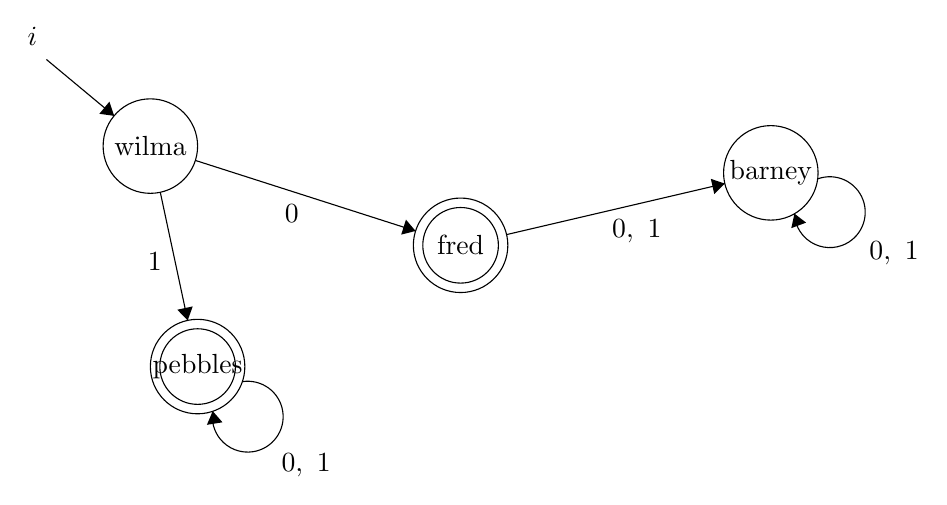
\begin{tikzpicture}[scale=0.2]
						\tikzstyle{every node}+=[inner sep=0pt]
						\draw [black] (17.3,-17.3) circle (3);
						\draw (17.3,-17.3) node {wilma};
						\draw [black] (37,-23.6) circle (3);
						\draw (37,-23.6) node {fred};
						\draw [black] (37,-23.6) circle (2.4);
						\draw [black] (56.7,-19) circle (3);
						\draw (56.7,-19) node {barney};
						\draw [black] (20.3,-31.3) circle (3);
						\draw (20.3,-31.3) node {pebbles};
						\draw [black] (20.3,-31.3) circle (2.4);
						\draw [black] (10.7,-11.8) -- (15,-15.38);
						\draw (10.15,-10.36) node [left] {$i$};
						\fill [black] (15,-15.38) -- (14.7,-14.48) -- (14.06,-15.25);
						\draw [black] (20.16,-18.21) -- (34.14,-22.69);
						\fill [black] (34.14,-22.69) -- (33.53,-21.97) -- (33.23,-22.92);
						\draw (26.28,-20.99) node [below] {$0$};
						\draw [black] (17.93,-20.23) -- (19.67,-28.37);
						\fill [black] (19.67,-28.37) -- (19.99,-27.48) -- (19.01,-27.69);
						\draw (18.05,-24.65) node [left] {$1$};
						\draw [black] (23.13,-32.26) arc (99:-189:2.25);
						\draw (25.6,-37.55) node [right] {$0,\mbox{ }1$};
						\fill [black] (21.26,-34.13) -- (20.89,-35) -- (21.88,-34.84);
						\draw [black] (39.92,-22.92) -- (53.78,-19.68);
						\fill [black] (53.78,-19.68) -- (52.89,-19.38) -- (53.11,-20.35);
						\draw (48.19,-21.95) node [below] {$0,\mbox{ }1$};
						\draw [black] (59.663,-19.386) arc (110.30993:-177.69007:2.25);
						\draw (62.93,-24.08) node [right] {$0,\mbox{ }1$};
						\fill [black] (58.2,-21.59) -- (58,-22.51) -- (58.94,-22.16);
					\end{tikzpicture}
				\end{center}

				You follow the arrows through the states, as necessary, and if you end up on a final state then the element is in the language.
				\\ \\
				We prefer total functions to partial functions. We add a new state, which we'll call ``barney'', that acts as a black hole. A finite automaton only needs one black hole, where all states loop back to itself. We can always make $T$ total by directing transitions that are not otherwise specified to the black hole. The black hole state is \emph{not} a final state.
				\\ \\
				We can name our states whatever we'd like on our bubble diagram. Intelligent names should be chosen, like ``start'', ``zero'', ``nonzero'', and ``fail'', for instance.
				\\ \\
				Fun fact: regular languages have been proven to be closed under intersection and set difference. \lecture{February 6, 2013}
				\\ \\
				We sometimes denote a DFA as $\text{DFA} = < \Sigma, S, i, f, T >$.
				\\ \\
				For simplicity's sake, we'll setup some notation we'll be using to discuss DFAs. This is by convention only.
				\begin{itemize}
					\item $a, b, c, d$ (and other letters at the beginning of the standard alphabet) represent symbols in $\Sigma = \{a, b, c, d\}$.
					\item Particular strings are a concatenation of symbols from $\Sigma$. Some examples are $abca, bbca,$ and $\epsilon$ (the empty string).
					\item $x, y, z$ (and other letters near the end of the standard alphabet) are variables that represent strings. For example, let $x = abc$, then $x = x_0 x_1 x_2 \ldots x_{n - 1}$ where $n = |x|$.
				\end{itemize}
				The \textbf{DFA algorithm} is pretty simple. Given an input $x$ (which is implicitly a DFA = $< \Sigma, S, i, f, T >$, where $T$ is a total function), the output of the algorithm will be:
				\begin{align*}
					\begin{cases}
						\text{``accept''} & x \in L \\
						\text{``reject''} & x \not \in L
					\end{cases}
				\end{align*}
				The DFA algorithm is as follows: \\ \\
				\begin{algorithm}[H]
					state = i\;
					\For{$a = x_0, x_1, x_2, \ldots, x_{n - 1}$}{
						state = T[state, a]\;
					}
					\lIf{state $\in $ f}{accept}
					\lElse{reject}
				\end{algorithm}
				\vspace{0.5cm}
				The bonus question on A5 involves implementing this algorithm. You may want to use an array or map. It's the easiest bonus question all term.

				\begin{ex}
					We're given the binary integers, $\Sigma = \{ 0, 1 \}, S = \{ \text{start}, \text{zero}, \text{nonzero}, \text{error} \}, i = \text{start}, f = \{ \text{zero}, \text{nonzero} \}$, and function $T$ defined by: \\
					\begin{center}
						\begin{tabular}{|c|c|}
							\hline $S \times \Sigma$ & $S$ \\ \hline
							start, 0 & zero \\
							start, 1 & nonzero \\
							zero, 0 & error \\
							zero, 1 & error \\
							nonzero, 0 & nonzero \\
							nonzero, 1 & nonzero \\
							error, 0 & error \\
							error, 1 & error \\ \hline
						\end{tabular}
					\end{center}
					This table for $T$ isn't very intuitive. Let's look at the bubble diagram representing this DFA for a clearer picture.
					
					\begin{center}
						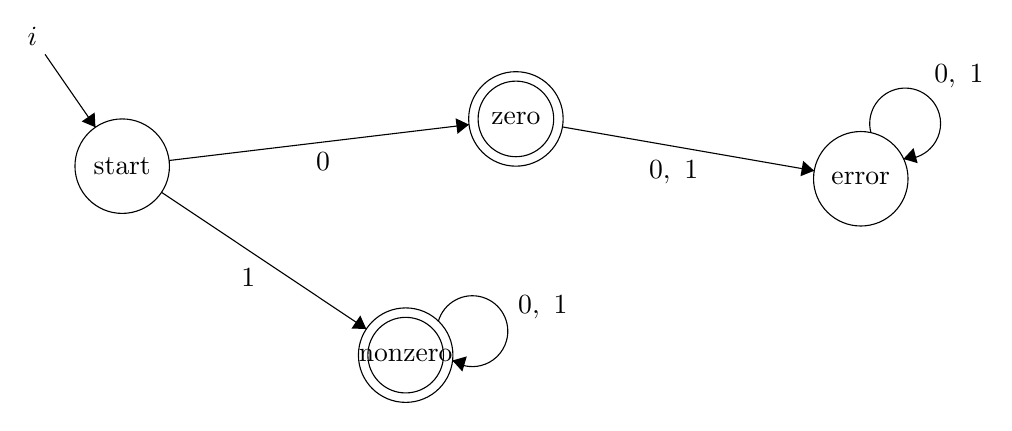
\begin{tikzpicture}[scale=0.2]
							\tikzstyle{every node}+=[inner sep=0pt]
							\draw [black] (13,-15.7) circle (3);
							\draw (13,-15.7) node {start};
							\draw [black] (38,-12.7) circle (3);
							\draw (38,-12.7) node {zero};
							\draw [black] (38,-12.7) circle (2.4);
							\draw [black] (59.9,-16.5) circle (3);
							\draw (59.9,-16.5) node {error};
							\draw [black] (31,-27.7) circle (3);
							\draw (31,-27.7) node {nonzero};
							\draw [black] (31,-27.7) circle (2.4);
							\draw [black] (15.5,-17.36) -- (28.5,-26.04);
							\fill [black] (28.5,-26.04) -- (28.12,-25.18) -- (27.56,-26.01);
							\draw (21,-22.2) node [below] {$1$};
							\draw [black] (33.075,-25.549) arc (163.75996:-124.24004:2.25);
							\draw (38.11,-24.64) node [right] {$0,\mbox{ }1$};
							\fill [black] (33.97,-28.04) -- (34.6,-28.74) -- (34.88,-27.78);
							\draw [black] (15.98,-15.34) -- (35.02,-13.06);
							\fill [black] (35.02,-13.06) -- (34.17,-12.66) -- (34.29,-13.65);
							\draw (25.76,-14.79) node [below] {$0$};
							\draw [black] (40.96,-13.21) -- (56.94,-15.99);
							\fill [black] (56.94,-15.99) -- (56.24,-15.36) -- (56.07,-16.34);
							\draw (48.02,-15.29) node [below] {$0,\mbox{ }1$};
							\draw [black] (60.547,-13.583) arc (195.22332:-92.77668:2.25);
							\draw (66.13,-10.74) node [above] {$0,\mbox{ }1$};
							\fill [black] (62.61,-15.24) -- (63.51,-15.51) -- (63.25,-14.55);
							\draw [black] (8.1,-8.6) -- (11.3,-13.23);
							\draw (7.3,-8.1) node [above] {$i$};
							\fill [black] (11.3,-13.23) -- (11.25,-12.29) -- (10.43,-12.86);
						\end{tikzpicture}
					\end{center}

					Let's look at \underline{x = 10}. x = 10 will execute the following: \\
					\begin{algorithm}[H]
						state = start\;
						state = T[start, 1]; // state = nonzero \\
						state = T[nonzero, 0]; // state = nonzero \\
						(end loop) \\
						nonzero $\in $ f? Yes, accept.
					\end{algorithm}
					\vspace{0.5cm}
					Next, let's look at \underline{x = 01}. x = 01 will execute the following: \\
					\begin{algorithm}[H]
						state = start\;
						state = T[start, 0]; // state = zero \\
						state = T[zero, 1]; // state = error \\
						(end loop) \\
						error $\in $ f? No, reject.
					\end{algorithm}
				\end{ex}

				\begin{ex}
					Let's construct a finite automaton that represents the MIPS assembly notation for registers.
					\\ \\
					Given $\Sigma = \{ \$, 0, 1, 2, 3, 4, 5, 6, 7, 8, 9 \}, L = $ MIPS assembly notation for registers (i.e. $\{ \$0, \$1, \$2, \ldots, \$31 \}$).
					\\ \\
					It's useful to name your DFA states with what you've learned so far based on the conditions that led to that state, because that's the only way we know what we've determined in the past. These names don't matter, but it'll make the finite automaton much easier for you to understand.
					\\ \\
					We're going to assume there is an error state that all undefined transitions lead to. We'll make this assumption in general in this course. You need to draw the error state only when you need a \emph{total} function $T$ (such as when you intend to run the DFA algorithm), or when you're explicitly asked to draw it.
					\\ \\
					Let's look at the bubble diagram for this finite automaton that represents the notation of MIPS registers.
					\begin{center}
						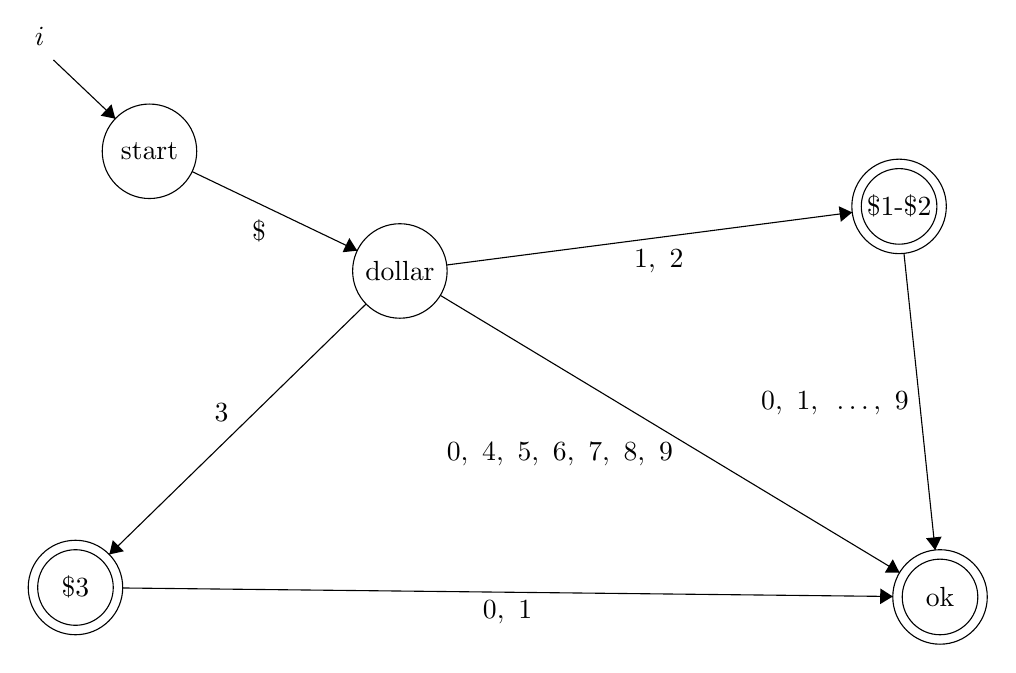
\begin{tikzpicture}[scale=0.2]
							\tikzstyle{every node}+=[inner sep=0pt]
							\draw [black] (11.8,-10.2) circle (3);
							\draw (11.8,-10.2) node {start};
							\draw [black] (27.7,-17.8) circle (3);
							\draw (27.7,-17.8) node {dollar};
							\draw [black] (62,-38.5) circle (3);
							\draw (62,-38.5) node {ok};
							\draw [black] (62,-38.5) circle (2.4);
							\draw [black] (59.4,-13.7) circle (3);
							\draw (59.4,-13.7) node {\$1-\$2};
							\draw [black] (59.4,-13.7) circle (2.4);
							\draw [black] (7.1,-37.9) circle (3);
							\draw (7.1,-37.9) node {\$3};
							\draw [black] (7.1,-37.9) circle (2.4);
							\draw [black] (5.7,-4.4) -- (9.63,-8.13);
							\draw (5.17,-2.93) node [left] {$i$};
							\fill [black] (9.63,-8.13) -- (9.39,-7.22) -- (8.7,-7.94);
							\draw [black] (14.51,-11.49) -- (24.99,-16.51);
							\fill [black] (24.99,-16.51) -- (24.49,-15.71) -- (24.06,-16.61);
							\draw (18.76,-14.51) node [below] {\$};
							\draw [black] (59.71,-16.68) -- (61.69,-35.52);
							\fill [black] (61.69,-35.52) -- (62.1,-34.67) -- (61.11,-34.77);
							\draw (60.05,-26.2) node [left] {$0,\mbox{ }1,\mbox{ }\dots,\mbox{ }9$};
							\draw [black] (10.1,-37.93) -- (59,-38.47);
							\fill [black] (59,-38.47) -- (58.21,-37.96) -- (58.19,-38.96);
							\draw (34.54,-38.72) node [below] {$0,\mbox{ }1$};
							\draw [black] (25.55,-19.9) -- (9.25,-35.8);
							\fill [black] (9.25,-35.8) -- (10.17,-35.6) -- (9.47,-34.89);
							\draw (16.38,-27.37) node [above] {$3$};
							\draw [black] (30.68,-17.42) -- (56.42,-14.08);
							\fill [black] (56.42,-14.08) -- (55.57,-13.69) -- (55.7,-14.68);
							\draw (44.14,-16.43) node [below] {$1,\mbox{ }2$};
							\draw [black] (30.27,-19.35) -- (59.43,-36.95);
							\fill [black] (59.43,-36.95) -- (59,-36.11) -- (58.49,-36.96);
							\draw (37.86,-28.66) node [below] {$0,\mbox{ }4,\mbox{ }5,\mbox{ }6,\mbox{ }7,\mbox{ }8,\mbox{ }9$};
						\end{tikzpicture}
					\end{center}
					
					Every MIPS register must start with the dollar sign (\$). Keep in mind that only $\$0, \ldots, \$31$ are valid MIPS registers. So, if the next number is a 1 or a 2, we can have any second digit (from 0-9) to form a valid MIPS register. If the number is 3, we can only follow that up by a 0 or 1 (\$30 and \$31). We also need to handle all other single digit registers (\$0, \$4, \$5, \$6, \$7, \$8, \$9).
					\\ \\
					We could've made this differently by having multiple ``ok'' states, but those aren't necessary so all valid registers point to the same ``ok'' state in this diagram. We can point all complete paths to a single complete state because what happens from the complete state onwards does not differ. In this case, all complete states have no further path (except to an implied black hole), and all complete states are final states, so having one complete state (denoted ``ok'' on the bubble diagram) is acceptable.
					\\ \\
					In general, you can combine two states if everything that follows from that point is the same among all of the states you're combining.
				\end{ex}
				[This lecture is incomplete. Will finish typesetting later today.]
\end{document}
